\section{Preliminary cryptographic concepts}

\subsection{Hash functions}
A hash function is a fuction that maps an arbitrary long input string to a fixed
length output string. Let $h$ refer to an hash function of length $n$:

\[
  h\colon \{0,1\}^* \to \{0,1\}^n
\]

$m$ is usually called ``the message'', while $d$ is usually called ``the digest``
and it can be seen as a compact representation of m. The length of $d$ is the
length of the hash.

Hash functions are usually used to provide data integrity and they're also used to
construct other cryptographic primitives such as MACs and digital signatures.

\subsubsection{Desired properties}
An hash function should ideally meet these properties:
\begin{itemize}
  \item \textbf{Computational efficiency}: given m, it must be easy to compute ${d=h(m)}$
  \item \textbf{Preimage resistance} (also called \textbf{one-way property}):
  given ${d=h(m)}$, it must be computationally infeasible computing $m$ ($m$ is the
  preimage)
  \item \textbf{Weak collision resistance} (also called
  \textbf{2\textsuperscript{nd} preimage resistance}): given $m_1$ and ${d_1=h(m_1)}$,
  it must be computationally infeasible finding a $m_2 \neq m_1$ so that ${h(m_2)=d_1}$
  \item \textbf{Strong collision resistance}: it must be computationally infeasible
  finding paris of distinct and colliding messages. Two messages $m_1\neq m_2$
  collide when ${h(m_1)=h(m_2)}$.
  \item \textbf{Avalanche effect}: changing a single bit of $m$ should cause every
  bit of ${d=h(m)}$ to change with probability ${P=0.5}$
\end{itemize}

\subsubsection{Examples of hash functions}
\begin{itemize}
  \item \textbf{MD5}: published in 1991, it's a 128-bit hash function that was
  used for file integrity checks. Today it's considered unsecure and it shouldn't
  be used anymore.
  \item \textbf{Secure Hash algorithm 1 (SHA-1)}: 160-bit hash function that was
  used in SSL and TLS implementations. Today is considered unsecure and it's
  deprecated.
  \item \textbf{SHA-2}: family of SHA functions which includes SHA-256, SHA-384
  and SHA-512. SHA-256 is currently used in several parts of the Bitcoin network.
  \item \textbf{SHA-3}: latest family of SHA functions, it is a NIST-standardized
  version of Keccak, which uses a new approach called ``sponge construction''
  instead of the Merkle-Damgard transformation previously used. This family
  includes SHA3-256, SHA3-384 and SHA3-512.
\end{itemize}

\subsubsection{Design of SHA-256}

\subsubsection{Message Authentication Codes (MACs)}
A MAC is an hash function which uses a key and which can therefore be used to
provide both integrity and authentication (proof of origin). Authentication is
based on a key pre-shared between the sender and the receiver. The receiver can
verify both integrity and authentication of a message by computing the MAC function
of the message and comparing it with the one received from the sender: if they are the
same then integrity and authentication are confirmed (note that it is assumed that
only the sender and the receiver know the key).

MAC functions can be constructed using block ciphers or hash functions:
\begin{itemize}
  \item in the first approach, block ciphers are used in the Cipher block chaining mode (CBC mode):
  the MAC of a message will be the output of the last round of the CBC operation.
  The length of MAC in this case is the same as the block length of the block cipher
  used to generate it.
  \item In the second approach they key is hashed with the message using a certain
  construction scheme. The most simple ones are \emph{suffix-only} and
  \emph{prefix-only}, which however are weak and vulnerable:
  \begin{itemize}
    \item suffix-only: ${d=MAC_k(m)=h(m|k)}$, where $h$ is an hash function
    \item prefix-only: ${d=MAC_k(m)=h(k|m)}$, where $h$ is an hash function
  \end{itemize}
\end{itemize}





\subsection{Digital signature}
Digital signatures are used to associate a message with the entity from which the
message has been originated. They provide the same service as MACs (authentication
and non-repudiation) plus the non-repudiation.

Digital signature is based on public key cryptography: Alice can sign a message
by encrypting it using its private key. Usually however, for efficiency and security
reasons, Alice doesn't encrypt the message but its digest (hash of the message).
Figure \ref{fig:digital-signature} shows how a generical digital signature function
works.

An example of digital signature algorithms are RSA and ECDSA.

\begin{figure}[!htb]
	\centering
	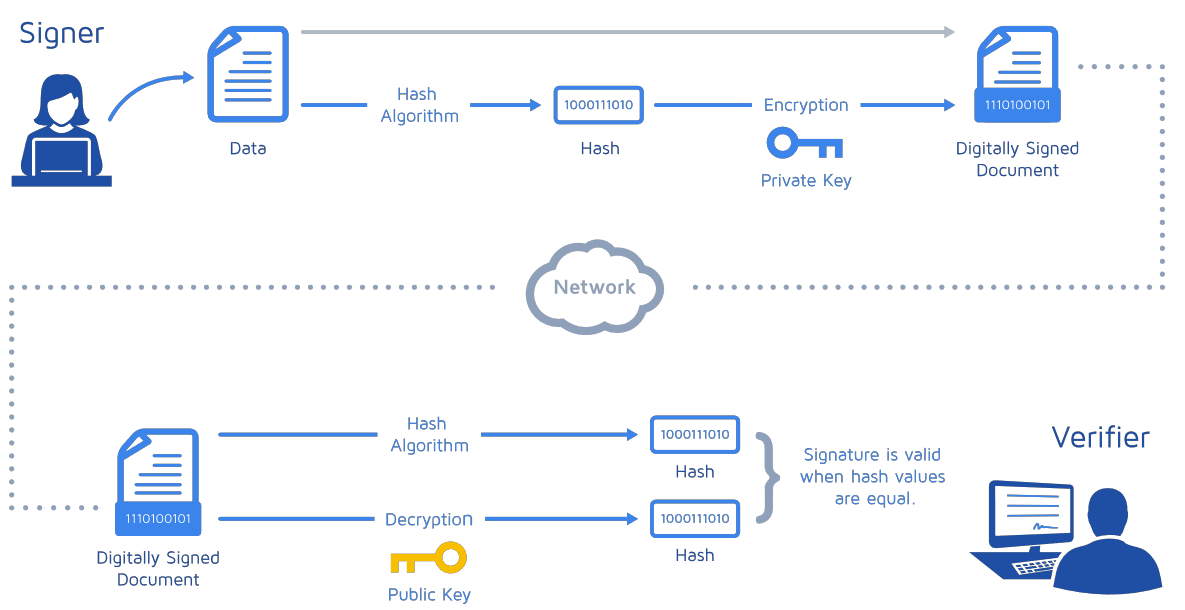
\includegraphics[width=1\linewidth]{img/digital-signature.png}
	\caption{digital signature signing and verification scheme}
	\label{fig:digital-signature}
\end{figure}





\subsection{Elliptic Curve Digital Signature Algorithm (ECDSA)}
ECDSA is a variant of the Digital Signature Algorithm (DSA) which uses elliptic
curve cryptography.

\subsubsection{Key pair generation}
\begin{enumerate}
  \item Define an elliptic curve $E$ with modulus $P$, coefficients $a$ and $b$ and a
  generator point $G$ that forms a cyclic group of order $p$, with $p$ prime
  \item Choose a random integer $d$ so that ${0 < d < q}$
  \item Compute the public key $B$ so that ${B = d A}$
\end{enumerate}
The public key is the sextuple ${K_{pb} = (p,a,b,q,A,B)}$, while the private key
is the value of $d$ randomly chosen in Step 2: ${K_{pr} = d}$

\subsubsection{Signing a message}
\begin{enumerate}
  \item Choose an ephemeral key $K_e$, where ${0 < K_e < q}$.
  It should be ensured that $K_e$ is truly random and no two signatures have the same key
  because otherwise the private key can be calculated
  \item Compute ${R = K_e A}$
  \item Initialize a variable $r$ with the x coordinate value of the point $R$
  \item The signature on the message $m$ can be calculated as follow:
  \[{S=(h(m)+dr)K_e^{-1}\mod q}\]
\end{enumerate}
